\appendix{Представление графического материала}

Графический материал, выполненный на отдельных листах,
изображен на рисунках А.1--А.\arabic{числоПлакатов}.
\setcounter{числоПлакатов}{0}

\renewcommand{\thefigure}{А.\arabic{figure}} % шаблон номера для плакатов

\begin{landscape}

\begin{плакат}
    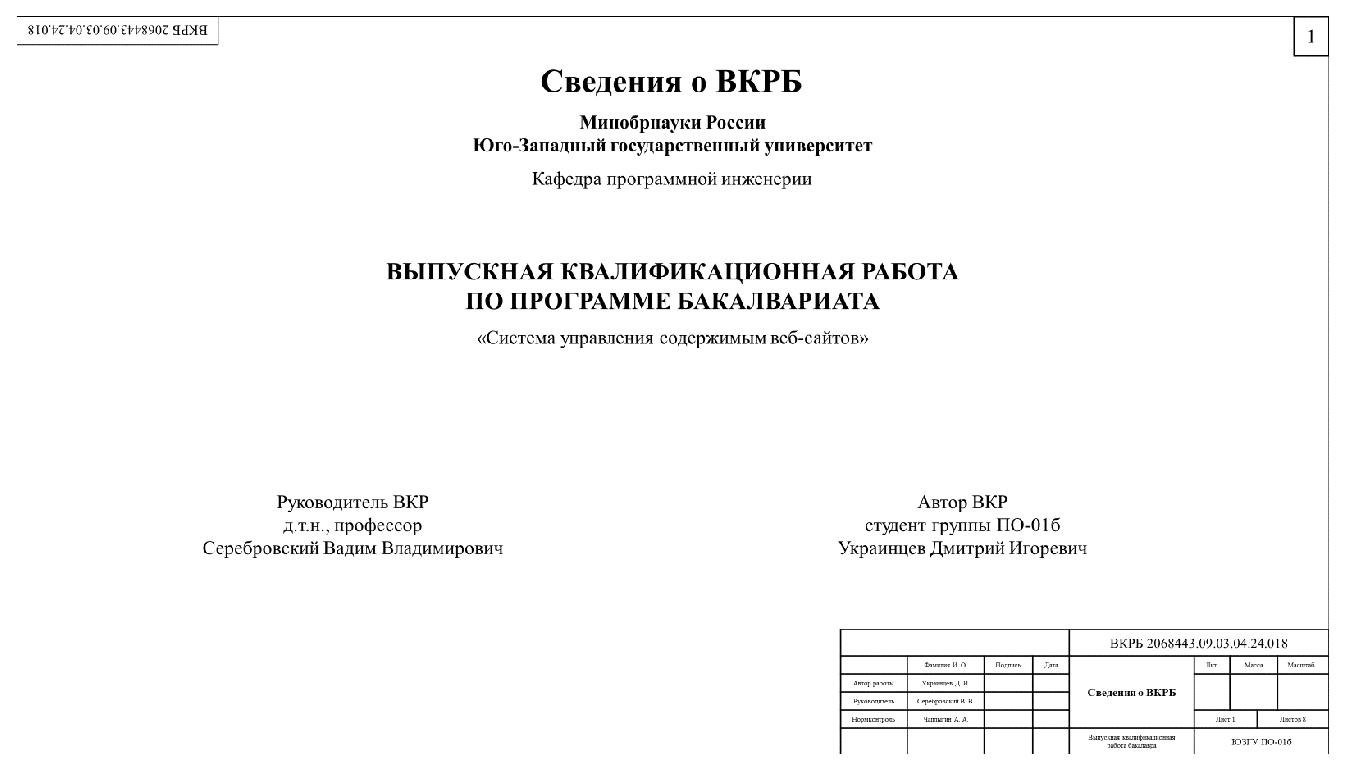
\includegraphics[width=0.82\linewidth]{плакат1.eps}
    \заголовок{Сведения о ВКРБ}
    \label{pl1:image}      
\end{плакат}

\begin{плакат}
    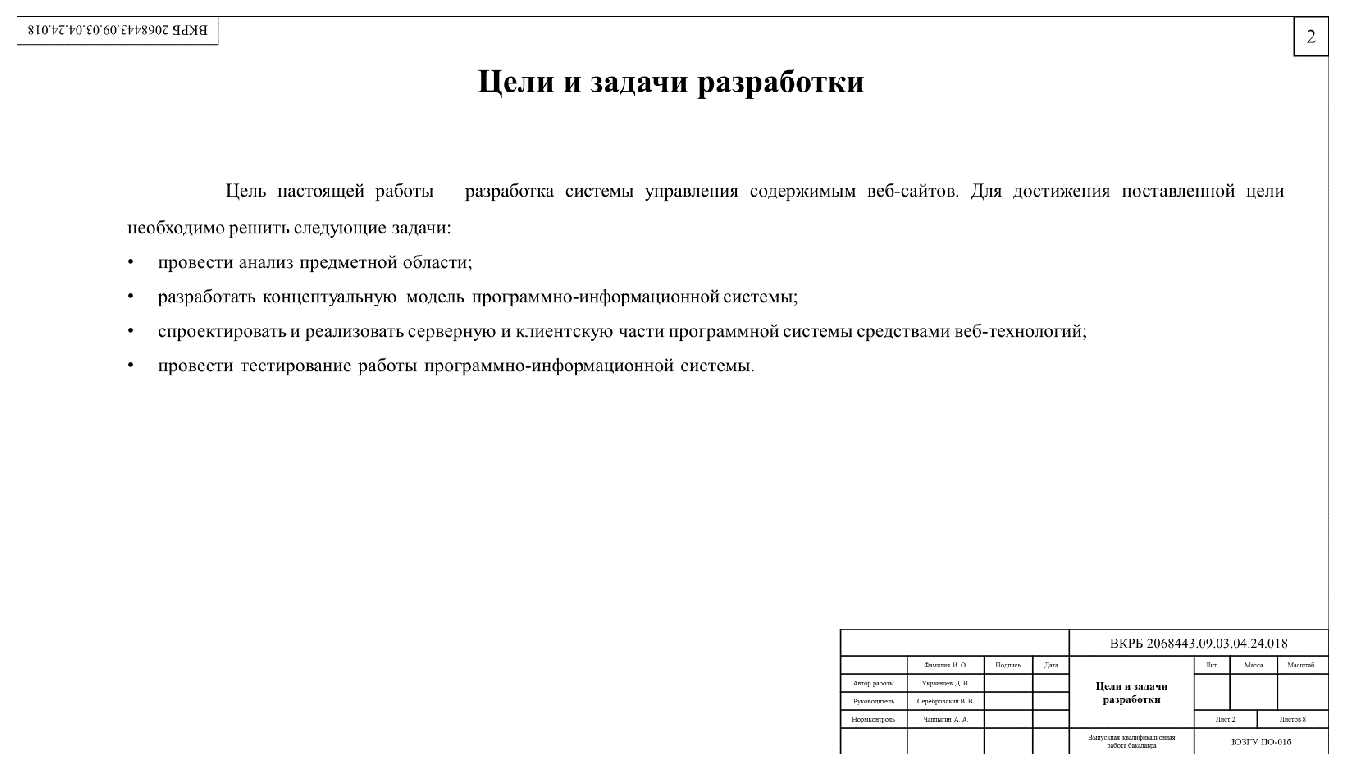
\includegraphics[width=0.82\linewidth]{плакат2.eps}
    \заголовок{Цели и задачи разработки}
    \label{pl2:image}      
\end{плакат}

\begin{плакат}
    \includegraphics[width=0.82\linewidth]{плакат3.eps}
    \заголовок{Диаграмма прецедентов}
    \label{pl3:image}      
\end{плакат}

\begin{плакат}
	\includegraphics[width=0.82\linewidth]{плакат4.eps}
	\заголовок{Реляционная модель данных}
	\label{pl4:image}      
\end{плакат}

\begin{плакат}
	\includegraphics[width=0.82\linewidth]{плакат5.eps}
	\заголовок{Диаграмма компонентов}
	\label{pl5:image}      
\end{плакат}

\begin{плакат}
	\includegraphics[width=0.82\linewidth]{плакат6.eps}
	\заголовок{Диаграмма классов (часть 1)}
	\label{pl6:image}      
\end{плакат}

\begin{плакат}
	\includegraphics[width=0.82\linewidth]{плакат7.eps}
	\заголовок{Диаграмма классов (часть 2)}
	\label{pl7:image}      
\end{плакат}

\begin{плакат}
	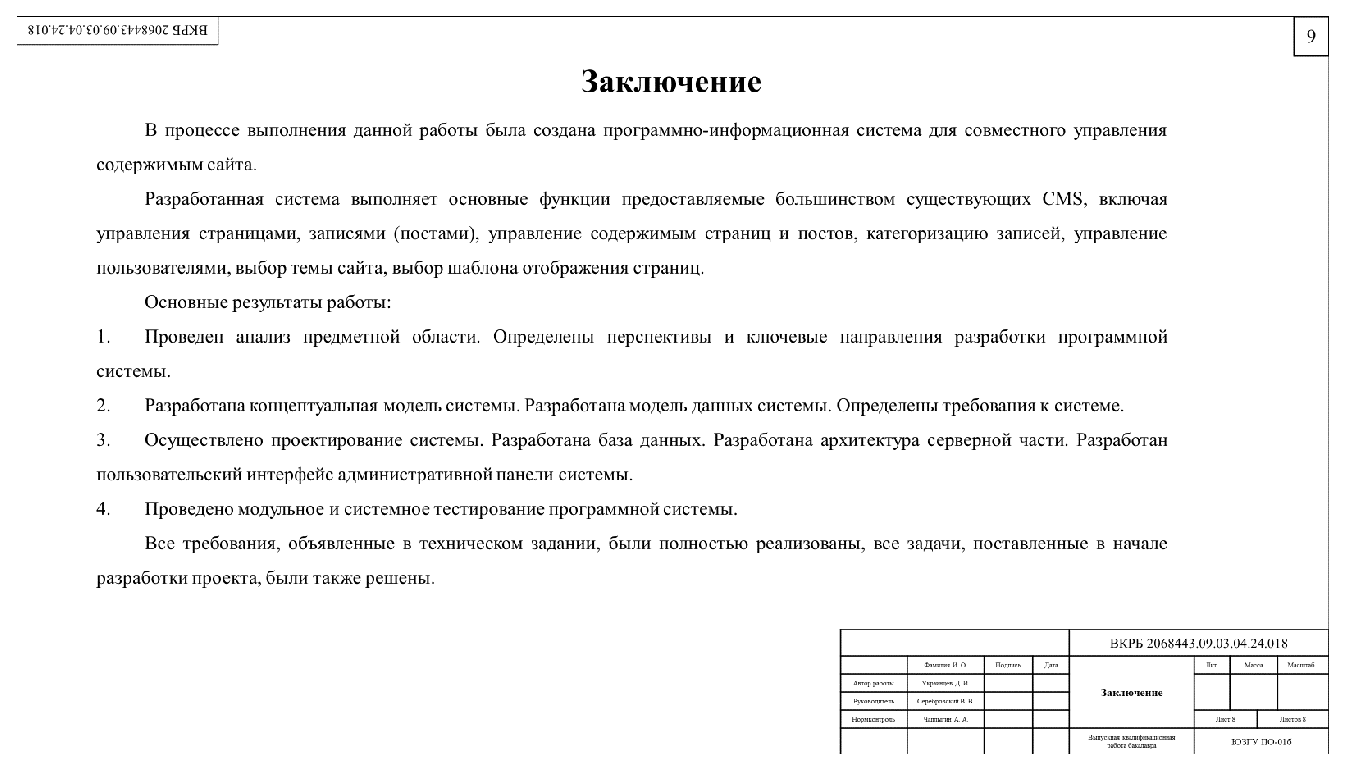
\includegraphics[width=0.82\linewidth]{плакат8.eps}
	\заголовок{Заключение}
	\label{pl8:image}      
\end{плакат}

\end{landscape}
